\documentclass[a5paper,titlepage,11pt,openany]{scrbook}
\usepackage[a5paper,backref]{hyperref}
\usepackage[papersize={148.5mm,215mm},twoside,bindingoffset=0.5cm,hmargin={1cm,1cm},
				vmargin={2cm,2cm},footskip=1.1cm,driver=dvipdfm]{geometry}
\usepackage{palatino}
\usepackage[utf8]{inputenc}

\usepackage{pstricks}
\usepackage{graphicx}
\usepackage[bahasa]{babel} 
\usepackage{lettrine}
\usepackage{pifont}
\usepackage{enumitem}
\usepackage{wrapfig}
\usepackage{indentfirst}
\usepackage{parcolumns}
\usepackage[titles]{tocloft}
\usepackage{longtable}
\usepackage{microtype}
\usepackage{hyphenat}
\usepackage{xparse}


\renewcommand{\cftchapfont}{%
  \fontsize{9}{8}\selectfont
}

\makeatletter
\renewcommand{\@pnumwidth}{1em} 
\renewcommand{\@tocrmarg}{1em}
\makeatother

\author{Lingkungan St. Petrus Maguwo}
\title{Warta Iman}
\setlength{\parindent}{1cm}
\psset{unit=1mm}


\begin{document}
\thispagestyle{empty}
\thispagestyle{empty}
\newcommand{\edisi}[1]{%
\DeclareFixedFont{\PT}{T1}{ppl}{b}{}{0.7in}
\DeclareFixedFont{\PTit}{T1}{ppl}{b}{it}{0.7in}
\DeclareFixedFont{\PTsmall}{T1}{ppl}{b}{it}{0.25in}
\DeclareFixedFont{\PTsmaller}{T1}{ppl}{b}{it}{0.175in}
\DeclareFixedFont{\PTsmallest}{T1}{ppl}{b}{it}{0.15in}

\begin{pspicture}(14cm,2cm)
\rput[rb](10.35cm,3cm){\PTsmallest {#1}}
\rput[lb](-2cm,1.5cm){\PT {WARTA IMAN}}
\rput[lb](0cm,0.5cm){\PTsmall {Lingkungan St. Petrus Maguwo}}
\end{pspicture}%
}

\newcounter{kgkcounter}[chapter]
\renewcommand{\thekgkcounter}{\arabic{kgkcounter}. }
\newcommand{\kgk}[1]{\refstepcounter{kgkcounter}\textbf{\flushleft \textbf{\thekgkcounter #1}}\\}

\newcommand{\kutipan}[1]{%
\noindent{\framebox{\parbox{10cm}{\centering\emph{#1}}}}}

\edisi{November 2011}

%\vspace{1cm}

\begin{center}
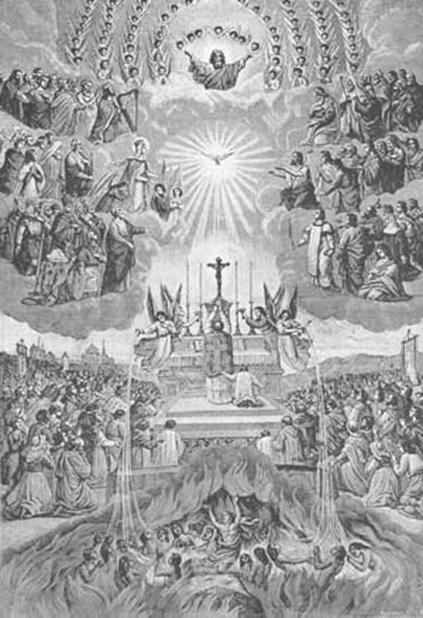
\includegraphics[scale=0.85]{gambar/purgatory2.jpg}
\end{center}

%\vspace{1cm}

\begin{center}
{\PTsmaller {Kasih, kerendahan hati, dan menurut pada kehendak Allah }}
\end{center}

\setlength{\parindent}{1cm}
\pagestyle{plain}
\begin{center}
%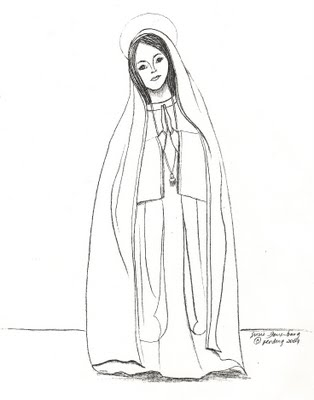
\includegraphics[scale=0.25]{gambar/Mary-Coloring-5.jpg}
\end{center}
\chap{Hari Raya Semua Orang Kudus dan Peringatan Arwah Semua Orang Beriman\\
\small \emph{Romo William P. Saunders} \normalsize}

\kutipan{Dapatkah dijelaskan asal mula Hari Raya Semua Orang Kudus dan Peringatan Arwah Semua Orang Beriman? Apakah kedua perayaan tersebut ada hubungannya dengan paham kekafiran dan perayaan Halloween?}
\sumber{seorang pembaca di Springfield}


Keduanya, Hari Raya Semua Orang Kudus dan Peringatan Arwah Semua Orang Beriman, berkembang dalam kehidupan Gereja, terlepas dari paham kekafiran dan perayaan Halloween.

Marilah pertama-tama kita membahas Hari Raya Semua Orang Kudus. Asal mula yang tepat dari perayaan ini tidak diketahui dengan pasti, walau, sesudah disahkannya kekristenan pada tahun 313 M, suatu peringatan umum demi menghormati para kudus, khususnya para martir, muncul di berbagai wilayah di segenap penjuru Gereja. Sebagai contoh di Timur, kota Edessa merayakan pesta ini pada tanggal 13 Mei; Siria merayakannya pada hari Jumat sesudah Paskah; kota Antiokhia merayakannya pada hari Minggu pertama sesudah Pentakosta. Baik St Efrem (wafat 373) dan St Yohanes Krisostomus (wafat 407) menegaskan akan adanya perayaan ini dalam khotbah mereka. Di Barat, suatu peringatan demi menghormati semua orang kudus juga dirayakan pada hari Minggu pertama sesudah Pentakosta. Alasan utama menetapkan suatu pesta umum ini adalah karena kerinduan untuk menghormati sejumlah besar martir, teristimewa yang wafat dalam masa penganiayaan oleh Kaisar Diocletion (284-305), yaitu masa penganiayaan yang paling luas, keji dan bengis. Singkatnya, tidak akan ada cukup hari dalam satu tahun apabila masing-masing martir dirayakan tersendiri, lagipula kebanyakan dari para martir ini wafat dalam kelompok. Sebab itu, suatu pesta umum bagi semua orang kudus, dianggap paling tepat.

Pada tahun 609, Kaisar Phocas memberikan Pantheon di Roma (= kuil yang dipersembahkan bagi semua dewa) kepada Paus Bonifasius IV, yang mempersembahkannya kembali pada tanggal 13 Mei di bawah nama St Maria ad Martyres (atau St Maria dan Semua Martir). Apakah Bapa Suci dengan sengaja memilih tanggal 13 Mei karena tanggal perayaan yang populer ini telah ditetapkan di Timur atau apakah hal ini sekedar kebetulan belaka, tak seorang pun tahu pasti.

Penetapan tanggal 1 November sebagai Hari Raya Semua Orang Kudus berkembang seturut berjalannya waktu. Paus Gregorius III (731-741) mempersembahkan suatu oratorium di Basilika St Petrus yang asli demi menghormati semua orang kudus pada tanggal 1 November (setidaknya demikian menurut beberapa catatan), maka kemudian tanggal ini menjadi tanggal resmi untuk merayakan Hari Raya Semua Orang Kudus di Roma. St. Beda (wafat 735) mencatat HR Semua Orang Kudus dirayakan pada tanggal 1 November di Inggris, dan perayaan serupa juga ada di Salzburg, Austria. Ado dari Vienne (wafat 875) menceritakan bagaimana Paus Gregorius IV meminta Raja Louis yang Saleh (778-840) untuk memaklumkan tanggal 1 November sebagai HR Semua Orang Kudus di seluruh wilayah Kekaisaran Romawi yang Kudus. Buku Doa Misa dari abad ke-9 dan ke-10 juga menempatkan HR Semua Orang Kudus dalam penanggalan liturgi pada tanggal 1 November.

Menurut seorang sejarahwan Gereja perdana, John Beleth (wafat 1165), Paus Gregorius IV (827-844) secara resmi memaklumkan tanggal 1 November sebagai HR Semua Orang Kudus, memindahkannya dari tanggal 13 Mei. Tetapi, Sicard dari Cremona (wafat 1215) mencatat bahwa Paus Gregorius VII (1073-85) akhirnya menghapus tanggal 13 Mei dan mengamanatkan 1 November sebagai tanggal perayaan HR Semua Orang Kudus. Secara keseluruhan dapat kita lihat bahwa Gereja menetapkan perayaan liturgis demi menghormati para kudus ini sama sekali terlepas dari pengaruh kekafiran.

Sekarang, kita membahas hubungannya dengan perayaan Halloween. Tanggal 1 November menandai Samhain, yaitu dimulainya musim dingin bangsa Celtic. (Bangsa Celtic hidup sekitar 2000 tahun yang lalu di Inggris, Scotlandia, Wales, Irlandia dan Perancis utara.) Samhain, yang namanya dipakai sebagai nama perayaan, adalah dewa kematian bangsa Celtic, namanya secara harafiah berarti “akhir musim panas”. Karena musim dingin adalah masa-masa dingin, kegelapan dan kematian, kaum Celtic segera menghubungkannya dengan kematian manusia. Malam menjelang Samhain, yaitu tanggal 31 Oktober, adalah saat kurban kafir bangsa Celtic, dan Samhain mengijinkan jiwa-jiwa orang mati untuk kembali ke rumah-rumah duniawi mereka pada malam ini. Setan-setan, hantu, roh dan tukang sihir datang untuk mencelakai manusia, teristimewa orang-orang yang pernah menyakiti mereka semasa mereka masih hidup. Kucing, juga, dianggap keramat sebab dianggap dulunya mereka adalah manusia yang dikutuk sebagai hukuman atas perbuatan-perbuatan jahat mereka semasa di dunia.

Guna melindungi diri dari roh-roh jahat yang bergentayangan pada malam Samhain, orang-orang memadamkan perapian mereka, dan para Druids (para imam dan guru rohani bangsa Celtic) mendirikan suatu api unggun tahun baru yang sangat besar terbuat dari dahan-dahan pohon oak yang keramat. Druids mempersembahkan kurban-kurban bakaran - hasil bumi, hewan, bahkan manusia - dan menyampaikan ramalan mengenai tahun yang akan datang dengan memeriksa sisa-sisa kurban bakaran. Orang-orang terkadang mengenakan kostum dari kepala dan kulit binatang. Dari api unggun yang baru ini, perapian rumah para penduduk sekali lagi dinyalakan.

Kelompok-kelompok etnis yang berbeda masing-masing memiliki adat mereka sendiri yang berbaur dengan perayaan. Di Irlandia, orang mengadakan suatu arak-arakan demi menghormati dewa Muck Olla. Mereka mengikuti sang pemimpin yang mengenakan jubah putih dengan topeng dari kepala binatang dan minta sedekah makanan. (Irlandia juga merupakan asal dari dongeng `jack-o-lantern': seorang bernama Jack yang tak dapat masuk ke surga karena kikir, namun ia juga tak dapat masuk ke neraka karena ia sering melontarkan lelucon untuk mengolok-olok iblis; jadi ia dihukum untuk berjalan mengelilingi dunia dengan lenteranya hingga tiba Hari Penghakiman.)

Orang-orang Scotlandia berjalan menyusuri padang dan desa-desa dengan membawa suluh dan menyalakan api unggun guna menghalau tukang sihir dan roh-roh jahat.

Di Wales, setiap orang meletakkan suatu batu yang telah ditandai pada api unggun yang sangat besar. Jika batu miliknya tak dapat diketemukan kembali keesokan paginya, maka pastilah orang itu akan mati dalam tahun itu.

Di samping tradisi Celtic yang telah ada, penjajah Romawi yang berkuasa atas Inggris pada tahun 43 M membawa serta dua perayaan kafir lainnya: Feralia yang dirayakan di penghujung bulan Oktober demi menghormati mereka yang telah meninggal dunia; dan suatu perayaan pada musim gugur demi menghormati Pomona, dewi buah-buahan dan pepohonan, kemungkinan, melalui perayaan ini, buah apel kemudian dihubungkan dengan perayaan Halloween. Unsur-unsur perayaan Romawi ini dipadukan dengan perayaan Samhain bangsa Celtic.

Dengan tersebar luasnya kekristenan dan dengan ditetapkannya HR Semua Orang Kudus, sebagian dari tradisi-tradisi kafir ini tetap tinggal dalam wilayah yang masyarakatnya berbahasa Inggris, dalam perayaan All Hallows Eve (atau Halloween, All Saints Eve, Malam menjelang HR Semua Orang Kudus), kemungkinan pertama-tama memang berasal dari takhayul, tetapi kemudian, lebih pada unsur sukaria tanpa ada hubungan dengan kekafiran. Oleh sebab itulah, anak-anak kecil (dan juga sebagian orang dewasa) masih mengenakan berbagai macam kostum dan malam itu berpura-pura menjadi setan, tukang sihir, drakula, monster, ninja, bajak laut, dan lain sebagainya, tanpa lagi memikirkan kekafiran. Dengan demikian, HR Semua Orang Kudus jelas muncul dari devosi Kristiani yang sejati, terlepas dari paham kekafiran.

Sejalan dengan Hari Raya Semua Orang Kudus, berkembang pula Peringatan Arwah Semua Orang Beriman. Gereja tak henti-hentinya mendorong umat beriman untuk mempersembahkan doa-doa dan Misa Kudus bagi jiwa-jiwa umat beriman yang telah meninggal dunia, yang masih berada di purgatorium. Pada saat kematian mereka, jiwa-jiwa ini belum bersih sepenuhnya dari dosa-dosa ringan atau belum melunasi hutang dosa di masa lalu, dan oleh sebab itu belum dapat menikmati kebahagiaan surgawi. Umat beriman di dunia dapat menolong jiwa-jiwa di api penyucian ini agar dapat segera menikmati kebahagiaan surgawi melalui doa-doa, perbuatan-perbuatan baik dan mempersembahkan Misa Kudus bagi jiwa-jiwa menderita ini.

Pada masa-masa Gereja awali, nama-nama umat beriman yang telah meninggal dunia ditempelkan di Gereja sehingga komunitas akan mengenangkan mereka dalam doa. Pada abad keenam, biara-biara Benediktin mengadakan peringatan khidmad akan para anggota yang telah meninggal dunia, pada hari-hari sesudah Pentakosta. Di Spanyol, St Isidorus (wafat 636) menegaskan adanya perayaan pada hari Sabtu sebelum Minggu Sexagesima (Minggu kedua sebelum Masa Prapaskah, kedelapan sebelum Paskah, dalam penanggalan kuno). Di Jerman, Widukind, Abbas Corvey (wafat 980) mencatat adanya suatu upacara khusus pada tanggal 1 Oktober bagi umat beriman yang telah meninggal dunia. St Odilo, Abbas Cluny (wafat 1048) mengamanatkan kepada seluruh biara Cluniac agar doa-doa khusus dipanjatkan dan Ofisi bagi Yang Meninggal dimadahkan demi segenap jiwa-jiwa di purgatorium, pada tanggal 2 November, sehari sesudah HR Semua Orang Kudus. Benediktin dan Kartusian menerapkan devosi yang sama, dan segera saja tanggal 2 November dirayakan sebagai Peringatan Arwah Semua Orang Beriman di segenap Gereja.

Tradisi-tradisi lainnya muncul dalam perjalanan waktu sehubungan dengan perayaan Peringatan Arwah Semua Orang Beriman. Pada abad ke-15, Dominikan menetapkan suatu tradisi di mana setiap imam mempersembahkan tiga Misa Kudus pada Peringatan Arwah Semua Orang Beriman. Paus Benediktus XIV pada tahun 1748 menyetujui praktek ini dan devosi ini dengan cepat menyebar ke seluruh Spanyol, Portugis dan Amerika Latin. Dalam masa Perang Dunia I, Paus Benediktus XV, menyadari akan banyaknya mereka yang tewas akibat perang dan begitu banyak Misa yang tak dapat dipersembahkan karena hancurnya gereja-gereja, memberikan hak istimewa kepada segenap imam untuk mempersembahkan tiga Misa Kudus pada Peringatan Arwah Semua Orang Beriman: satu untuk intensi khusus, satu untuk arwah semua orang beriman, dan satu untuk intensi Bapa Suci.

Tradisi-tradisi lainnya berkembang sehubungan dengan Peringatan Arwah Semua Orang Beriman. Di Meksiko, sanak-saudara merangkai karangan-karangan bunga dan dedaunan, juga membuat salib-salib dari bunga-bunga segar maupun bunga-bunga kertas beraneka warna guna diletakkan pada makam sanak-saudara yang telah meninggal, di pagi hari Peringatan Arwah Semua Orang Beriman. Keluarga akan menghabiskan sepanjang hari itu di pemakaman. Imam akan mengunjungi makam, menyampaikan khotbah dan mempersembahkan doa-doa bagi mereka yang meninggal, serta memberkati makam-makam satu per satu. Permen “Tengkorak” dibagikan kepada anak-anak.

Praktek serupa didapati pula di Louisiana. Sanak-saudara membersihkan serta melabur batu-batu nisan, mempersiapkan karangan-karangan bunga dan dedaunan, juga salib-salib dari bunga-bunga segar maupun bunga-bunga kertas untuk menghiasi makam. Pada siang hari Peringatan Arwah Semua Orang Beriman, imam berarak sekeliling makam, memberkati makam-makam dan mendaraskan rosario. Lilin-lilin dinyalakan dekat kubur pada senja hari; satu untuk setiap anggota keluarga yang telah meninggal dunia. Pada Peringatan Arwah Semua Orang Beriman, biasanya Misa dirayakan di pemakaman. Dua contoh praktek kebudayaan ini berpusat pada pentingnya mengenangkan mereka yang telah meninggal dunia serta mendoakan jiwa-jiwa mereka.

Namun demikian, pada Abad Pertengahan, suatu kepercayaan takhayul, mungkin pengaruh dari paham kafir bangsa Celtic, mengatakan bahwa jiwa-jiwa di api penyucian menampakkan diri pada Peringatan Arwah Semua Orang Beriman sebagai tukang sihir, kodok, hantu, dll kepada mereka yang telah berbuat salah terhadap mereka semasa mereka masih hidup di dunia. Oleh sebab itu, beberapa kelompok etnis juga mempersiapkan makanan sesaji guna menjamu dan menenangkan roh-roh pada hari itu. Praktek-praktek semacam ini kemungkinan merupakan sisa-sisa perayaan Samhain bangsa Celtic seperti yang dibicarakan di atas. Pada masa sekarang, makanan sajian seperti itu tidak lagi ada hubungannya dengan kekafiran melainkan lebih sebagai wujud penitensi.  

Oleh sebab itu, baik Hari Raya Semua Orang Kudus maupun Peringatan Arwah Semua Orang Beriman, berasal dari kepercayaan kristiani dan muncul dalam kehidupan Gereja melalui spiritualitas yang sehat. Segala praktek seputar kedua perayaan religius ini, yang berasal dari paham kafir - seperti Halloween - telah lama kehilangan makna kekafirannya.


* Fr. Saunders is is pastor of Our Lady of Hope Church in Potomac Falls.
sumber : “Straight Answers: All Saints and All Souls Day” by Fr. William P. Saunders; Arlington Catholic Herald, Inc; Copyright ©2004 Arlington Catholic Herald. All rights reserved; www.catholicherald.com
Diperkenankan mengutip / menyebarluaskan artikel di atas dengan mencantumkan: “diterjemahkan oleh YESAYA: www.indocell.net/yesaya atas ijin The Arlington Catholic Herald.”
	
	                                                                                                                                                                                                                                                                                                            	
\chap{Paranormal dan Penyihir: Apa Kata Kitab Suci?\\
\small \emph{Romo William P. Saunders} \normalsize}

Belakangan ini, saya melihat banyak iklan di televisi yang menawarkan jasa paranormal. Ada juga tayangan TV mengenai Sabrina, si gadis penyihir. Bagaimanakah kita, sebagai umat Kristiani, menyikapi masalah ini?
~ seorang pembaca di McLean

Sebagai orang Katolik, kita ingat bahwa perintah Allah yang pertama mengatakan, “Akulah TUHAN, Allahmu. Jangan ada padamu allah lain di hadapan-Ku.” Ketika ditanya hukum manakah yang terutama, Tuhan kita Yesus Kristus, dengan mengulang perintah yang ada dalam Kitab Ulangan, mengatakan, “Kasihilah Tuhan, Allahmu, dengan segenap hatimu dan dengan segenap jiwamu dan dengan segenap akal budimu” (Mat 22:37). Sementara Tuhan, menurut kehendak-Nya, dapat mewahyukan masa depan kepada para nabi atau para kudus, kita sebagai pribadi wajib senantiasa percaya akan penyelenggaraan ilahi-Nya. St Paulus mengingatkan kita, “Kita tahu sekarang, bahwa Allah turut bekerja dalam segala sesuatu untuk mendatangkan kebaikan bagi mereka yang mengasihi Dia, yaitu bagi mereka yang terpanggil sesuai dengan rencana Allah” (Rm 8:28). Mungkin terkadang kita juga memiliki rasa ingin tahu tentang apa yang akan terjadi di masa mendatang, namun demikian kita mengandalkan hidup kita pada Tuhan, percaya penuh akan kasih sayang dan pemeliharaan-Nya.

Berusaha mengetahui masa depan dengan membaca tangan, kartu ramal, atau bentuk-bentuk ramalan lainnya, atau berusaha mengendalikan masa depan melalui black magic, ilmu gaib atau sihir, merupakan pelanggaran terhadap perintah Allah yang pertama. Kitab Suci banyak mengutuk praktek-praktek ini: dalam Perjanjian Lama kita dapati, “Seorang ahli sihir perempuan janganlah engkau biarkan hidup” (Kel 22:18), “Siapa yang mempersembahkan korban kepada allah kecuali kepada TUHAN sendiri, haruslah ia ditumpas.” (Kel 22:20). “Apabila seorang laki-laki atau perempuan dirasuk arwah atau roh peramal, pastilah mereka dihukum mati, yakni mereka harus dilontari dengan batu dan darah mereka tertimpa kepada mereka sendiri” (Im 20:27), dan “Di antaramu janganlah didapati seorangpun yang mempersembahkan anaknya laki-laki atau anaknya perempuan sebagai korban dalam api, ataupun seorang yang menjadi petenung, seorang peramal, seorang penelaah, seorang penyihir, seorang pemantera, ataupun seorang yang bertanya kepada arwah atau kepada roh peramal atau yang meminta petunjuk kepada orang-orang mati. Sebab setiap orang yang melakukan hal-hal ini adalah kekejian bagi TUHAN….” (Ul 18:10-12).

Perjanjian Baru juga membicarakan masalah ini: Dalam Kisah Para Rasul, di Filipi St Paulus bertemu dengan seorang hamba perempuan “yang mempunyai roh tenung” yang mendapatkan penghasilan besar dengan tenungan-tenungannya. St Paulus membebaskannya dari roh jahat itu (Kis 16:16 dst). Dalam ayat-ayat lain, kita dapati kutukan-kutukan terhadap sihir dan praktek-praktek gaib pada umumnya. St Paulus mengutuk seorang tukang sihir (Gal 5:20). Dalam Kisah Para Rasul, St Paulus mencela Elimas, tukang sihir, dan menyebutnya sebagai “anak Iblis, engkau musuh segala kebenaran” (Kis 13:8 dst). St Petrus mengecam Simon, si tukang sihir, yang bermaksud membeli kuasa Roh Kudus guna menjadikan diri lebih berkuasa (Kis 8:9 dst). Dalam Kitab Wahyu, Yesus memaklumkan, “Tetapi orang-orang penakut, orang-orang yang tidak percaya, orang-orang keji, orang-orang pembunuh, orang-orang sundal, tukang-tukang sihir, penyembah-penyembah berhala dan semua pendusta, mereka akan mendapat bagian mereka di dalam lautan yang menyala-nyala oleh api dan belerang; inilah kematian yang kedua” (Why 21:8).

Katekismus Gereja Katolik dalam menjelaskan perintah Allah yang pertama, mengulang kutukan terhadap praktek ramalan, “Segala macam ramalan harus ditolak: mempergunakan setan dan roh jahat, pemanggilan arwah atau tindakan-tindakan lain, yang tentangnya orang berpendapat tanpa alasan, seakan-akan mereka dapat `membuka tabir' masa depan. Di balik horoskop, astrologi, membaca tangan, penafsiran pratanda dan orakel (petunjuk gaib), paranormal dan menanyai medium, terselubung kehendak supaya berkuasa atas waktu, sejarah dan akhirnya atas manusia; demikian pula keinginan menarik perhatian kekuatan-kekuatan gaib. Ini bertentangan dengan penghormatan dalam rasa takwa yang penuh kasih, yang hanya kita berikan kepada Allah” (No. 2116). Segala praktek dengan mempergunakan kuasa-kuasa gaib dikutuk karena bertentangan dengan agama yang benar dan biasanya dianggap sebagai dosa berat. Segala bentuk permohonan kepada setan jelas merupakan dosa berat. (Perlu diperhatikan bahwa sekedar membaca horoskop di koran karena iseng bukanlah dosa berat; tetapi menganggapnya serius atau sengaja membayar demi mendapatkan ramalan adalah dosa).

Perhatian khusus perlu diberikan kepada sihir, yang menyangkut baik menyingkapkan masa depan maupun berusaha mengendalikan masa depan. Memang, dalam tayangan televisi, Sabrina atau tukang sihir satunya yang lebih senior dapat saja mengarang-ngarang cerita yang menyenangkan seputar dunia sihir dan ilmu sihir. Namun demikian, sihir menyangkut mengadakan sesuatu tertentu yang di luar kuasa normal manusia, dengan bantuan kuasa-kuasa (gaib) selain dari kuasa Allah. Pada umumnya, sihir menyangkut suatu perjanjian dengan setan, atau setidaknya memohon bantuan roh-roh jahat. Dunia sihir meliputi ritus membangkitkan orang mati, membangkitkan gairah dalam diri orang, dan mendatangkan bencana atau bahkan kematian atas musuh. Setanisme, secara istimewa, menghaturkan pemujaan kepada Penguasa Kegelapan, dan bahkan merayakan “Misa Hitam,” yang meniru-niru Misa kita tetapi penuh dengan tindakan sakrilegi dan hujat. Bahkan jika orang berbicara mengenai “white magic” atau “sihir baik,” pelakunya juga memohon pada kekuatan-kekuatan yang bukan berasal dari Tuhan.

Kita percaya, seperti yang ditulis St Yohanes, bahwa “Allah adalah kasih” (1 Yoh 4:16). “Karena begitu besar kasih Allah akan dunia ini, sehingga Ia telah mengaruniakan Anak-Nya yang tunggal, supaya setiap orang yang percaya kepada-Nya tidak binasa, melainkan beroleh hidup yang kekal” (Yoh 3:16). Yesus adalah terang dunia; terang itu bercahaya di dalam kegelapan dan kegelapan itu tidak menguasainya (Yoh 1:4-5). Yesus adalah jalan dan kebenaran dan hidup (Yoh 14:6). Memohon bantuan setan atau kuasa-kuasa lain, masuk dalam dunia gelap (gaib) guna mendapatkan pertolongan, atau berusaha merampas kuasa yang hanya dimiliki Allah Sendiri, adalah menantang kuasa Allah yang Mahakuasa. Bertindak demikian adalah berpaling dari Allah dan menempatkan jiwa kita sendiri dalam bahaya.


* Fr. Saunders is dean of the Notre Dame Graduate School of Christendom College and Pastor of Queen of Apostles Parish, both in Alexandria.
sumber : “Straight Answers: Psychics and Witches: What Scripture Says” by Fr. William P. Saunders; Arlington Catholic Herald, Inc; Copyright ©1997 Arlington Catholic Herald, Inc. All rights reserved; www.catholicherald.com
Diperkenankan mengutip / menyebarluaskan artikel di atas dengan mencantumkan: “diterjemahkan oleh YESAYA: www.indocell.net/yesaya atas ijin The Arlington Catholic Herald.”
	
	                                                                                                                                                                                                                                                                                                           
\chap{Untuk Pembebasan Jiwa-jiwa di Api Penyucian}

\kgk*{Bapa kami yang ada di surga.}
Kami mohon dengan rendah hati kepada-Mu, Bapa yang kekal, mahabaik dan maharahim, ampunilah jiwa-jiwa malang yang merupakan ciptaan-Mu juga, biarpun mereka tidak mengasihi-Mu, telah menolak-Mu dan tidak menghormati-Mu. Demi pertobatan dan penebusan, kami persembahkan kepada-Mu pengorbanan semua kebajikan Putera-Mu terkasih, Tuhan kami, Yesus Kristus.

\kgk*{Dimuliakanlah nama-Mu.}
Kami mohon dengan rendah hati kepada-Mu, Bapa yang kekal, mahabaik dan maharahim, ampunilah jiwa-jiwa malang yang tidak memuliakan nama kudus-Mu dan sering menyalahgunakannya. Demi pertobatan dan penebusan, kami persembahkan kepada-Mu pengorbanan semua perkataan yang telah diucapkan oleh Putera-Mu, Tuhan kami, Yesus Kristus semasa hidupnya di dunia untuk memuliakan nama-Mu.

\kgk*{Datanglah kerajaan-Mu.}
Kami mohon dengan rendah hati kepada-Mu, Bapa yang kekal, mahabaik dan maharahim, ampunilah jiwa-jiwa malang yang tidak mempunyai hasrat dan kasih membara akan kerinduan pada kerajaan-Mu yang kudus. Demi pertobatan dan penebusan, kami persembahkan kepada-Mu pengorbanan semua kasih Putera-Mu, Tuhan kami, Yesus Kristus, yang menginginkan setiap insan diterima dalam kerajaan-Mu yang kudus.

\kgk*{Jadilah kehendak-Mu, di atas bumi seperti di dalam surga.}
Kami mohon dengan rendah hati kepada-Mu, Bapa yang kekal, mahabaik dan maharahim, ampunilah jiwa-jiwa malang yang tidak tunduk dengan tulus ikhlas pada kehendak-Mu yang kudus, tetapi yang sering mengikuti kehendaknya sendiri. Demi hati Ilahi Yesus dan kepatuhan-Nya yang besar.

\kgk*{Berilah kami rejeki pada hari ini, dan ampunilah kesalahan kami seperti kami pun mengampuni yang bersalah kepada kami.}
Kami mohon dengan rendah hati kepada-Mu, Bapa yang kekal, mahabaik dan maharahim, ampunilah jiwa-jiwa malang yang dibebani oleh dosa-dosa karena mereka tidak mengasihi musuh-musuhnya dan tidak ingin mengampuninya. Demi pertobatan dan penebusan, kami persembahkan kepada-Mu pengorbanan kata-kata kudus dari Putera-Mu terkasih, Tuhan kami, Yesus Kristus, seperti dikatakan-Nya pada kayu salib: Bapa, ampunilah mereka, karena mereka tidak tahu apa yang dilakukannya.

\kgk*{Dan janganlah masukkan kami ke dalam pencobaan.}
Kami mohon dengan rendah hati kepada-Mu, Bapa yang kekal, mahabaik dan maharahim, ampunilah jiwa-jiwa malang yang tidak berjuang melawan cobaan besar, tetapi mengalah pada godaan setan yang mempercepat kehancuran. Demi pertobatan dan penebusan, kami persembahkan kepada-Mu semua ketaatan, kerja keras dan semua penderitaan pahit serta kematian yang dialami Tuhan kami, Yesus Kristus.

\kgk*{Tetapi bebaskanlah kami dari yang jahat.}
Kami mohon dengan rendah hati kepada-Mu, Bapa yang kekal, mahabaik dan maharahim, ampunilah jiwa-jiwa malang dan hantarkanlah mereka bersama dengan Yesus Kristus pada kerajaan-Mu yang mulia karena Engkaulah kemuliaan itu.
\kgk*{Amin.}
\chap{7 Cara Menghindari Api Penyucian\\
 \small \emph{P. Josep Susanto Pr.} \normalsize}
	

Ketika kita masih muda dan sehat kita belum banyak memberi perhatian terhadap hidup setelah mati. Pikiran tentang sorga, neraka, Api penyucian belum mendominasi benak kita. Namun ketika orang sudah pensiun, mulai sakit-sakitan, atau tenaga sudah mulai loyo barulah mereka memberi perhatian serius akan nasibnya sesudah mati. Pikiran tentang surga atau Api penyucian akan mewarnai hari-hari mereka.

Masalah mulai datang ketika kita
berhadapan dengan fakta dalam kehidupan sehari-hari, kematian tidak pandang tua ataupun muda, bisa terjadi kapan saja, sehat atau sakit, laki-laki atau perempuan. Kutipan Kitab Suci ini bisa menyadarkan kita : “Apa gunanya seorang memperoleh seluruh dunia tetapi kehilangan nyawanya? Dan apakah yang dapat diberikannya sebagai ganti nyawanya? (Mat 16:26).  Karena itu “Carilah dahulu Kerajaan Allah, maka semuanya itu akan ditambahkan juga kepadamu” (Luk 12:31).

     Menurut ajaran Gereja, ada dua macam hukuman di Api Penyucian. Pertama, hukuman karena “perasaan kehilangan Tuhan”. Sedangkan yang kedua hukuman karena “sesal batin yang tak kunjung henti”. Hukuman karena kehilangan Tuhan diakibatkan oleh hilangnya kesempatan berjumpa dengan Allah, Sumber segala kebaikan, Tujuan dan Akhir hidup manusia. Sedangkan hukuman karena sesal batin yang tak kunjung henti menyangkut penderitaan yang dapat dirasakan sebagaimana halnya dengan hukuman fisik yang dapat kita rasakan.

     Setiap orang menerima hukuman sebanding dengan perbuatan yang dilakukan oleh seseorang selama hidup. Masing-masing orang harus mempertanggungjawabkan dosanya dihadapan Allah. Siksaan yang dijalani di dalam Api penyucian tidak bisa dibandingkan dengan penderitaan yang paling menyiksa yang ada di dunia ini. Hal itu digambarkan oleh Santo Thomas Aquinas dengan kalimat : Hukuman yang paling ringan di Api Punyucian beratnya melampaui semua penderitaan yang ada di dunia ini. Sejalan dengan itu Thomas A Kempis mengatakan : Satu jam penyiksaan lebih mengerikan dari pada seratus tahun menjalankan penebusan dosa yang keras yang kita lakukan di dunia ini. Hal itu dikarenakan, yang disiksa adalah “jiwa”, bukan sekedar “fisik”.

     Kiranya hal yang mengerikan yang terhadi di Api Penyucian memang berguna bagi kita untuk meningkatkan kualitas hidup kita lebih baik lagi di dunia ini, namun kita juga tidak boleh hidup dalam ketakuan saja. Karena hasil dari semua penyucian itu adalah kedamaian dan kebahagiaan abadi, sehingga kita bersatu kembali (pulang kembali) kepada Allah, Pemilik hidup kita. Jika pintu surga dan pintu Api penyucian dibuka, orang-orang yang meninggal akan segera memilih pintu Api Penyucian dari pada mereka menghadap Tuhan dengan noda dosa karena mereka melihat dirinya sendiri tidak pantas. Meraka akan menyucikan diri dengan kemauan mereka sendiri dan dengan penuh kasih, karena Api yang menyucikan mereka adalah api kasih yang berasal dari Allah sendiri.

\section*{Beberapa Kesaksian}

\subsection*{Santa Catharina dari Genoa (1447-1510)}

     Jiwa-jiwa akan mengalami kesengsaraan yang begitu dasyat sehingga tidak ada lidah yang dapat melukiskannya, atau sulit untuk dapat dimengerti sedikitpun sebelum Tuhan membuka rahasiaNya dengan rahmat istimewa.

\subsection*{Pastor Nieremberg (wafat 1658)} 

     Pada hari raya semua orang kudus, seorang gadis yang masih suci melihat penampakan di depan matanya, seorang wanita yang ia kenal, yang telah meninggal beberapa waktu sebelumnya. Sosok wanita itu berpakaian putih dengan kerudung di kepalanya, memegang rosario. Wanita yang telah meninggal itu sewaktu maish hidup pernah berjanji mempersembahkan Misa 3 kali di depan altar Santa Perawan Maria. Namun ia tidak melaksanakannya dalam hidup, sehingga hutang itu ditambahkan pada hukumannya. Sekarang ia meminta tolong gadis itu untuk mempersembahkan tiga kali Misa Kudus untuk dirinya. Gadis itu bersedia. Ketika Misa kudus yang ketiga sudah dirayakan arwah itu menampalkan diri lagi, mengungkapkan kegembiraan dan terima kasihnya. Arwah wanita itu selalu menampakan diri di depan Sakramen maha Kudus, melakuakan Pujian dan Penyembahan. Arwah itu terus menerus menampakan dirinya sampai saatnya tiba bagi dia naik ke surga diiring oleh malaikat pelindungnya. Awrah itu menyatakan bahwa dia sudah tidak menderita lagi atas hukuman “perasaan kehilangan Tuhan”, namun ia menambahkan bahwa kehilangan Tuhan itu menyebabkan dia menderita sengsara yang tak tertahankan.

\subsection*{Kesaksian seorang Bocah 11 tahun, Blasio Massei}           

     Pada suatu ketika seorang bocah 11 tahun menginggal dunia bernama Blasio Massei. Orang tuanya lalu berdevosi kepada Santo Bernardus dari Siena yang baru saja diangkat santo oleh Gereja Katolik. Orang tua Blassio mempersembahkan jiwa anaknya melalui santo ini. Ketika tubuh Blasio dibawa ke kubur, Blasio bangkit seolah-olah habis tidur nyenayak dan mengatakan bahwa Santo Bernardus telah menjadikannya hidup kembali, supaya menceritakan keajaiban yang telah diperintahkan santo.

     Blassio bercerita pada waktu dia meninggal, Santo Bernardus menampakan diri kepadanya. Santo itu menuntun tangannya dan berkata : Jangan takut, tetapi perhatikanlah apa yang kuperintahkan kepadamu, maka kamu harus mengingatnya dan setelah itu dapat menceritakannya.” Mereka mengunjungi Neraka, Api penyucian lalu sorga. Di neraka, Blassio melihat kengerian-kengerian yang tak terkatakan dan berbagai macam siksaan yang diberikan kepada mereka yang congkak, tamak, jahat, dan pendosa-pendosa lain.

     Di api penyucian, ia melihat siksaan yang paling menakutkan, ada berbagai macam hukuman menurut dosa yang dilakukan. Ia melihat ada arwah-arwah yang memohon kepadanya agar memberitahukan kepada sanak saudaranya, mereka merindukan dia permohonan dan perbuatan baik yang mereka lakukan.

     Di sorga, ia sangat terpesona. Ia melihat malaikat yang banyak sekali jumlahnya mengelilingi takhta Allah dan Perawan Maria yang Kudus.

\section*{7 Cara Menghindari Api Penyucian}
\begin{enumerate}
\item         Beriman Teguh pada Allah dan KerahimanNya
\item         Menghilangkan penyebabnya yaitu Dosa
\item         Devosi kepada Bunda Perawan Maria
\item         Membuat silih dengan amal kasih
\item         Rela menderita
\item         Menerima Sakramen-sakramen terutama Ekaristi dan Perminyakan orang sakit
\item         Menerima kematian dengan pasrah.
\end{enumerate}

\sumber{http://www.imankatolik.or.id}
%\chap{Warta Lingkungan}

\subsection*{APP}
Bulan Maret 2012 sudah masuk dalam masa Prapaskah. Sesuai dengan tradisi, setiap masa Prapaskah diadakan Aksi Puasa Pembangunan yang kegiatannya antara lain adalah ibadat APP di lingkungan. Untuk tahun ini Keuskupan Agung Semarang (KAS) menetapkan tema APP: \textit{Umat Katolik Sejati Harus Peduli dan Berbagi}. Dalam pelaksanaan di lingkungan St. Petrus, ibadat APP banyak diisi dengan \textit{sharing} yang mengacu pada buku panduan dari KAS.
Topik APP berawal dari baptis. Kapan kita dibaptis, kesan-kesan saat dibaptis, dan relevansinya dengan hidup menggereja dan bermasyarakat.

\subsection*{Misa pemberkatan rumah dan mitoni}
Bulan ini umat St. Petrus bertambah lagi dengan satu keluarga yang secara resmi bergabung sebagai warga lingkungan. Keluarga Bapak R. Mulyadi yang bertempat tinggal di Nanggulan, mengadakan misa syukur pemberkatan rumah dan sekaligus mitoni pada tanggal 22 Maret. Cicilia Nony Prayoga yang merupakan putri dari Bapak/Ibu Mulyadi menantikan kelahiran putranya bersama dengan suami tercinta
Bernadus Budhiprayoga.

Misa dipimpin oleh Rm. Albertus Purnomo, OFM yang merupakan kenalan baik keluarga R. Mulyadi saat masih di Jakarta. Dalam homilinya Romo menekankan bahwa Musa dapat melakukan tawar-menawar dengan Tuhan karena kedekatan Musa dengan Tuhan. Kenapa Musa dekat dengan Tuhan, karena Musa sering berdoa dan menaati perintah-Nya. Oleh karena itu kalau kita ingin dekat dengan Tuhan, maka rajin-rajinlah berdoa dan senantiasa menaati perintah-Nya.

\subsection*{Pendaftaran Krisma}
Telah diumumkan di gereja bahwa sakramen Krisma untuk paroki Marganingsih Kalasan akan dilangsungkan bulan September 2012. Calon penerima sakramen Krisma dapat mendaftarkan diri ke Ibu Munarti, Bapak Neo Suradi, atau kepada ketua lingkungan, dengan menyerahkan fotokopi surat baptis.

\hrule

\hrule
% SELECT day(`TglLahir`),
% concat(u1.`Baptis`,' ',u1.`Nama`) 
% FROM `umat` u1 WHERE month(TglLahir)=6 order by 1

%=========
% SELECT day(`TglNikah`),
% concat(u1.`Baptis`,' ',u1.`Nama`,' + ',u2.`Baptis`,' ',u2.`Nama`) 
% FROM `umat` u1 join kk on (u1.nokk=kk.id and u1.hubkel='KK')
%               join umat u2 on (u2.nokk=kk.id  and (u2.hubkel='istri' or u2.hubkel='isteri'))
% WHERE month(TglNikah)=1 order by 1

\section*{Yang berulang tahun kelahiran bulan ini}

\noindent{Semoga hari bahagia ini menguatkan imannya akan Dikau.}

\begin{longtable}{|c|l|} 
\hline
Tgl & Nama \\ \hline
\endhead1& Maria Rosary Sekar Seruni\\
5& Anna Maria Tri Henaningsih\\
6& Fransiscus Xaverius Sularto\\
7& Christina Sutarni\\
8& Marcellina Oktavia S. Padmini\\
11& Priscilla Oktiva Rossari\\
15& Yoseph Laba Atawolo\\
16& Ignatius Stanley Andi Pradana\\
18& Christina Sri Ning Hastuti\\
24& Margareta Maria Sri Pramuwati\\
25& Kristina Tri Tutwuri\\
\hline
\end{longtable}



\section*{Yang berulang tahun perkawinan  bulan ini}

Selamat ulang tahun perkawinan. Semoga keluarga-keluarga ini tumbuh menjadi keluarga Katolik yang sejati yang dibangun atas dasar iman dan kasih: kasih akan Dikau dan kasih antar semua anggota keluarga.

\begin{longtable}{|c|l|} 
\hline
Tgl & Keluarga \\ \hline
\endhead5& Nikolas Putut Andoko + Chatarina Krisyanti\\
6& Ignatius Luddy Indra Purnama + Anna Sri Wuryaningtyas\\
\hline
\end{longtable} 

\newpage
\chap{Kompendium Katekese Gereja Katolik}
\setcounter{kgkcounter}{61}
\small
\kgk{satu}

\flushright{(\dots \emph{bersambung} \dots)}
\normalsize
\end{document}